%%%%%%%%%%%%%%%%%%%%%%%%%%%%%%%%%%%%%%%%%
% Stylish Article
% LaTeX Template
% Version 2.2 (2020-10-22)
%
% This template has been downloaded from:
% http://www.LaTeXTemplates.com
%
% Original author:
% Mathias Legrand (legrand.mathias@gmail.com) 
% With extensive modifications by:
% Vel (vel@latextemplates.com)
%
% License:
% CC BY-NC-SA 3.0 (http://creativecommons.org/licenses/by-nc-sa/3.0/)
%
%%%%%%%%%%%%%%%%%%%%%%%%%%%%%%%%%%%%%%%%%

%----------------------------------------------------------------------------------------
%	PACKAGES AND OTHER DOCUMENT CONFIGURATIONS
%----------------------------------------------------------------------------------------

\documentclass[fleqn,11pt]{SelfArx} % Document font size and equations flushed left

\usepackage[spanish]{babel} % Specify a different language here - english by default
\usepackage{multirow}
\usepackage{lipsum} % Required to insert dummy text. To be removed otherwise

%----------------------------------------------------------------------------------------
%	COLUMNS
%----------------------------------------------------------------------------------------

\setlength{\columnsep}{0.55cm} % Distance between the two columns of text
\setlength{\fboxrule}{0.75pt} % Width of the border around the abstract

%----------------------------------------------------------------------------------------
%	COLORS
%----------------------------------------------------------------------------------------

\definecolor{color1}{RGB}{0,0,90} % Color of the article title and sections
\definecolor{color2}{RGB}{0,20,20} % Color of the boxes behind the abstract and headings

%----------------------------------------------------------------------------------------
%	HYPERLINKS
%----------------------------------------------------------------------------------------

\usepackage{hyperref} % Required for hyperlinks

\hypersetup{
	hidelinks,
	colorlinks,
	breaklinks=true,
	urlcolor=color2,
	citecolor=color1,
	linkcolor=color1,
	bookmarksopen=false,
	pdftitle={Title},
	pdfauthor={Author},
}

%----------------------------------------------------------------------------------------
%	ARTICLE INFORMATION
%----------------------------------------------------------------------------------------

\JournalInfo{Laboratorio de Electricidad y Magnetismo} % Journal information
\Archive{\textsuperscript\textcopyleft 2022 Ceballiguel} % Additional notes (e.g. copyright, DOI, review/research article)

\PaperTitle{MEDIDA DEL CICLO DE HISTÉRESIS DE UN MATERIAL FERROMAGNÉTICO} % Article title

\Authors{F. J. Ceballos\textsuperscript{1$\dagger$}, M. de Miguel\textsuperscript{1}*} % Authors
\affiliation{\textsuperscript{1}\textit{Facultad de CC. Físicas, Universidad Complutense de Madrid, Madrid, España}} % Author affiliation
\affiliation{\textsuperscript{$\dagger$}franceba@ucm.es,  *mdemig02@ucm.es} % Corresponding author

\Keywords{Sus --- Amongus --- Miguel} % Keywords - if you don't want any simply remove all the text between the curly brackets
\newcommand{\keywordname}{Keywords} % Defines the keywords heading name

%----------------------------------------------------------------------------------------
%	ABSTRACT
%----------------------------------------------------------------------------------------

\Abstract{}

%----------------------------------------------------------------------------------------

\begin{document}

\maketitle % Output the title and abstract box

\tableofcontents % Output the contents section

\thispagestyle{empty} % Removes page numbering from the first page

%----------------------------------------------------------------------------------------
%	ARTICLE CONTENTS
%----------------------------------------------------------------------------------------

\section*{Introducción} % The \section*{} command stops section numbering

\addcontentsline{toc}{section}{Introduction} % Adds this section to the table of contents



%------------------------------------------------

\section{Método experimental}

\begin{figure*}[ht]\centering % Using \begin{figure*} makes the figure take up the entire width of the page
	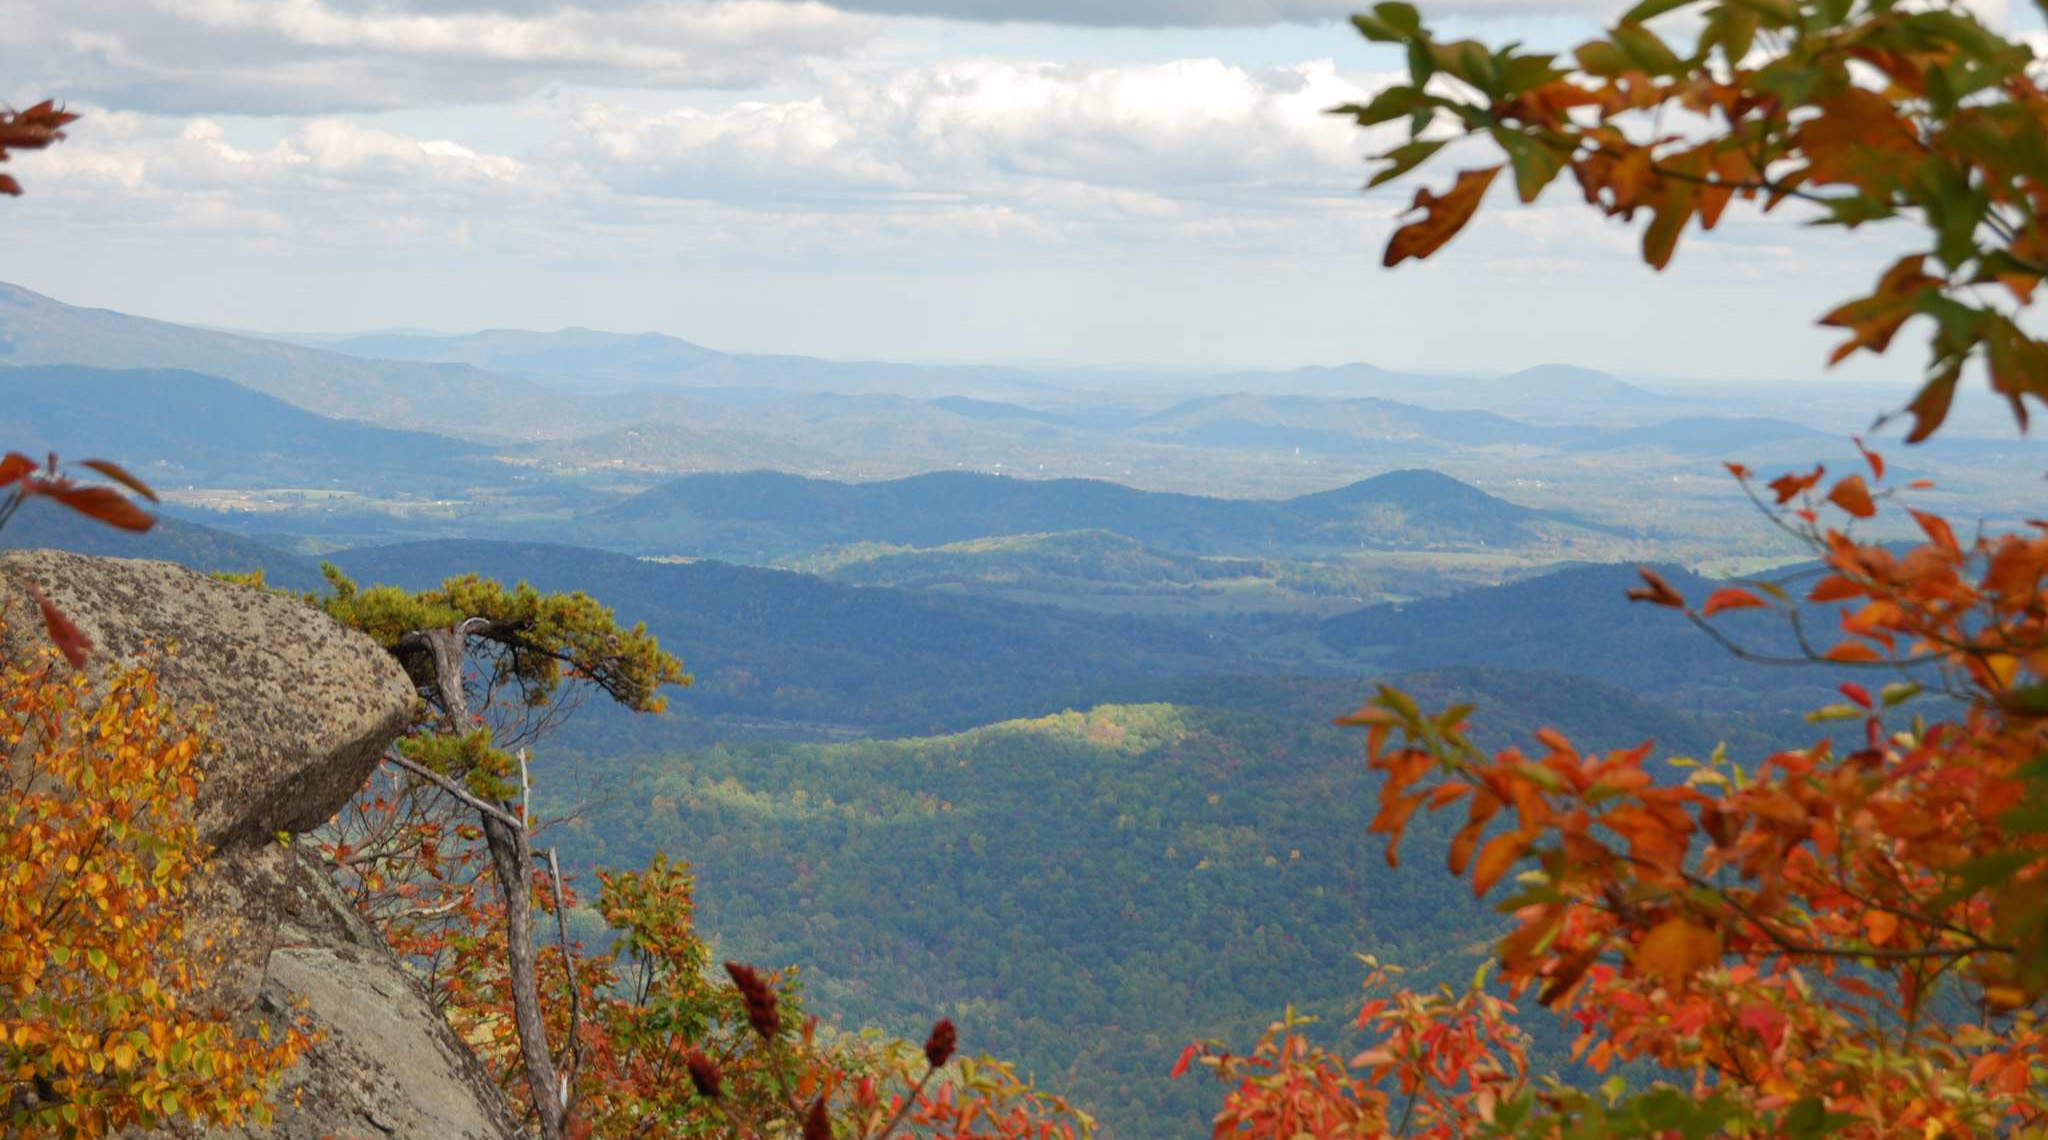
\includegraphics[width=\linewidth]{view}
	\caption{Wide Picture}
	\label{fig:view}
\end{figure*}

\lipsum[4] % Dummy text

\begin{equation}
	\cos^3 \theta =\frac{1}{4}\cos\theta+\frac{3}{4}\cos 3\theta
	\label{eq:refname2}
\end{equation}

\lipsum[5] % Dummy text

\begin{enumerate}[noitemsep] % [noitemsep] removes whitespace between the items for a compact look
	\item First item in a list
	\item Second item in a list
	\item Third item in a list
\end{enumerate}

\subsection{Subsection}

\lipsum[6] % Dummy text

\paragraph{Paragraph} \lipsum[7] % Dummy text
\paragraph{Paragraph} \lipsum[8] % Dummy text

\subsection{Subsection}

\lipsum[9] % Dummy text


%------------------------------------------------

\section{Resultados y análisis}
A continuación se mostrarán los resultados obtenidos a lo largo de la tarea. Todos los datos han sido tomados a través del programa COBRA Measure, de modo que las incertidumbres sistemáticas se han considerado iguales a la precisión provista por el mismo programa, siendo estas incertidumbres $\Delta H$ = 0.001 A m\textsuperscript{-1} o $\Delta B$ = 0.001 T, excepto en algunos casos concretos en los que se ha considerado podrían verse infravaloradas. En caso de tratarse de cálculos resueltos numéricamente no se han considerado incertidumbres al tratarse de resultados aproximados, especialmente en el caso de la derivada numérica necesaria para calcular la dependencia de la susceptibilidad magnética con la imanación. Las fórmulas empleadas para el cálculo de incertidumbres indirectas vienen indicadas donde son relevantes. 

\subsection{Ciclo de histéresis del núcleo de hierro macizo}
En primer lugar se realiza la medida de un ciclo del núcleo de Fe previamente desimanado a través del procedimiento descrito en la sección previa. Posteriormente, se toman medidas para voltajes suministrados entre 0 y 5V, invirtiendo el sentido del circuito para lograr los valores negativos y por ende ciclos cerrados. La curva obtenida se encuentra representada en la Figura siguiente.

\begin{figure}[ht!]\centering
	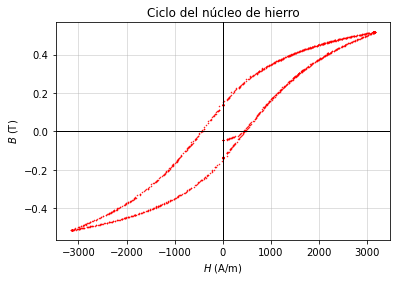
\includegraphics[width=\linewidth]{ciclofe}
	\caption{Ciclo de histéresis del núcleo de hierro}
	\label{fig:primerciclo}
\end{figure}

Se puede observar que para el rango de voltaje obtenido, la corriente a través de las bobinas no es suficiente para alcanzar la imanación de saturación, al menos de manera clara. En caso de que se alcanzase la saturación, se observarían rangos de $H$ en los que la inducción $B$ permanecería constante, tanto para $H >$ 0 como para $H <$ 0, es decir, la gráfica mostraría líneas horizontales de datos en los extremos del ciclo. \\

Si uno se fija en la curva de imanación inicial, esta no se observa exactamente como se esperaría, debido a que el núcleo no hubo sido totalmente desimanado en un principio. Se puede observar que para $H = 0$, $B < 0$, lo que implica que el hierro aún estaba ligeramente imanado. Esto provoca el solapamiento temprano de la curva de imanación inicial con el resto del ciclo. De tener el hierro completamente desimanado, se esperaría que la curva se solapase con el ciclo en un punto más cercano a la saturación.

\subsection{Campo coercitivo e imanación remanente}

A través de los datos graficados en la Figura \ref{fig:primerciclo}, se pueden estimar algunos puntos de interés del ciclo, como pueden ser la imanación remanente, es decir, la imanación que mantiene el material una vez se elimina el campo externo al que estaba sometido, o el campo coercitivo del núcleo, que sería el campo externo a aplicar para neutralizar la imanación del mismo. \\

La obtención de estos puntos se ha realizado de dos maneras: de manera directa, a través del propio programa de medidas y a partir de la gráfica del ciclo, estimando los cortes con los ejes del ciclo experimental. Se han tenido en cuenta valores tanto positivos como negativos. 

\begin{table}[htb!]
	\centering
	\begin{tabular}{c c c}
		%\hline
		\toprule
		& Measure & Python \\
		\midrule[0.7px]
		\multirow{2}{*}{$H_c$ (A/m)} & 441.537 $\pm$ 0.001 & 438 $\pm$ 11   \\
		& -442.106 $\pm$ 0.001 & -442.9 $\pm$ 6.4 \\
		\midrule
		\multirow{2}{*}{$B_r$ (mT)}& 136 $\pm$ 1 & 137 $\pm$ 1\\
		& -138 $\pm$ 1 & -138 $\pm$ 1 \\
		\midrule
		\multirow{2}{*}{$M_r$ (A/m)}& (108.23 $\pm$ 0.80) $\cdot 10^3$  & 109022.9 $\pm$ 1.0 \\
		& -(109.82  $\pm$ 0.80) $\cdot 10^3$  & -109816.1 $\pm$ 1.4  \\
		\bottomrule
	\end{tabular}
	\caption{Campo coercitivo $H_C$ e imanación remanente $M_r$ del núcleo de hierro}
	\label{remacitivo}
\end{table}

La incertidumbre de los datos proccesados con python ha sido considerada como la mayor distancia entre el punto crítico y el inmediatamente anterior o posterior a este. Por ejemplo, en la medida del campo positivo se tiene que, para una inducción entre -1 y 1 mT,  $H_c = 438.19$ (A/m). Ahora bien, la anterior medida de campo es  427.54 A/m ($B < -1$ mT), y la posterior 441.27 A/m ($B > 1$ mT), por lo que la incertidumbre será 438 - 427.54 = 10.65 $\approx$ 11 A/m. Las incertidumbres de $M_r$ obtenidas a través de los datos proporcionados por el programa de medida se han considerado:
\begin{equation}\label{incmr}
	\Delta M_r = \sqrt{\left(\frac{\Delta B}{\mu_0}\right)^2 + (\Delta H)^2} \approx \frac{\Delta B}{\mu_0},
\end{equation}
sin olvidar que $\Delta B$ y $\Delta H$ = 0.001 T o A/m, respectivamente.

Por último, aunque no se haya alcanzado un punto de saturación claro, se puede obtener el valor de los máximos de imanación del ciclo.

\begin{table}[htb!]
	\centering
	\begin{tabular}{c c c}
		%\hline
		\toprule
		& Measure & Python \\
		\midrule[0.7px]
		\multirow{2}{*}{$H_{max}$ (A/m)} & 3142.176 $\pm$ 0.001 & 3161.9 $\pm$ 8.9  \\
		& -3136.010 $\pm$ 0.001 & -3157.9 $\pm$ 7.9 \\
		\midrule
		\multirow{2}{*}{$B_{max}$ (mT)}& 512 $\pm$ 1 & 512 $\pm$ 1\\
		& -516 $\pm$ 1 & -516 $\pm$ 1 \\
		\midrule
		\multirow{2}{*}{$M_{max}$ (A/m)}& (404.29 $\pm$ 0.80) $\cdot 10^3$  & 404278.7 $\pm$ 1.3 \\
		& -(407.48  $\pm$ 0.80) $\cdot 10^3$  & -407457.9  $\pm$ 1.1  \\
		\bottomrule
	\end{tabular}
	\caption{Extremos del primer ciclo}
	\label{extremos}
\end{table}
Como se puede ver, en ambas Tablas \ref{remacitivo} y \ref{extremos} los valores obtenidos directamente desde la aplicación como los procesados con python son muy próximos entre sí, siendo los más desviados los valores del campo. 
  

\subsection{Estudio de la susceptibilidad magnética}
A partir de la curva de imanación inicial se puede estudiar la susceptibilidad magnética del material, $\chi$, la cual viene definida como 
\begin{equation}\label{susceptibility}
	\centering
	\chi = \frac{d M}{d H}.
\end{equation}
Para proceder con este cálculo, primero se ha procurado eliminar el ruido de las medidas de la curva de imanación inicial (con más de 200 puntos), reduciendo el número de puntos a 30 a través de una interpolación lineal.

\begin{figure}[ht!]\centering
	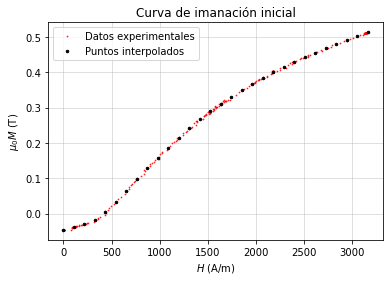
\includegraphics[width=\linewidth]{imanacioninicial}
	\caption{Curva de imanación inicial}
	\label{fig:imanacioninicial}
\end{figure}
Aplicando un algoritmo de diferenciación centrada a la muestra de puntos interpolados, tal que 
\begin{equation}
 \chi_i = \frac{1}{\mu_0} \frac{(\mu_0 M)_{i + 1} - (\mu_0 M)_{i - 1}}{H_{i + 1} - H_{i - 1}}
\end{equation}
se obtiene la siguiente curva para la susceptibilidad magnética del hierro.\footnote{En los cálculos con valores límite del conjunto se han reemplazado los las muestras $i - 1$ o $i + 1$ por las muestras $i$ según fuese necesario}
\begin{figure}[ht!]\centering
	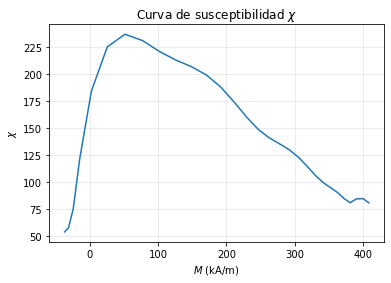
\includegraphics[width=\linewidth]{sus}
	\caption{Curva de susceptibilidad durante la imanación inicial}
	\label{fig:susceptibilidad}
\end{figure}

Observando la Figura \ref{fig:susceptibilidad}, se puede apreciar que la susceptibilidad en ningún momento llega a cero, lo que implica que la imanación del material depende del campo magnético externo a lo largo de toda la curva, es decir, no se alcanza el punto de saturación en ningún momento de la misma. \\

Se puede apreciar que el hierro ya presentó una susceptibilidad magnética $\chi_0$ = 53.9 antes de aplicar el campo y alcanzó su máximo $\chi_{max}$ = 237.8 para una imanación de $\approx$ 50 kA/m ($H \approx$ 650 A/m) en caso de haber alcanzado el punto de saturación, la susceptibilidad llegaría a ser cero para valores de $M$ superiores a los medidos.

\subsection{Permeabilidad relativa del hierro}
Empleando los mismos puntos interpolados para obtener la curva de susceptibilidad del metal, se puede analizar la evolución de la permeabilidad magnética relativa del núcleo, puesto que esta puede obtenerse como
\begin{equation}\label{permeabilidadrelativa}
	\mu_r = \frac{B}{\mu_0 H} = 1 + \frac{M}{H}.
\end{equation}

\begin{figure}[ht!]\centering
	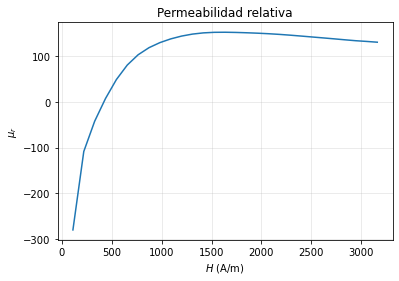
\includegraphics[width=\linewidth]{permeabilidad}
	\caption{Permeabilidad magnética relativa durante la imanación inicial}
	\label{fig:permeabilidad}
\end{figure}
Esta gráfica no constituye un resultado esperable, al menos en el primer tramo de la imanación. No obstante, hay que tener en cuenta que, como puede observarse en las Figuras \ref{fig:primerciclo} y \ref{fig:imanacioninicial}, hay un tramo inicial de la curva de histéresis en que el campo aplicado es positivo pero la imanación del material sigue siendo negativa. En este tramo (hasta $H \sim 500$ A/m), se puede observar que la permeabilidad relativa es consecuentemente negativa, pues el material se comporta somo si produjese una imanación opuesta al campo al que se somete. Sin embargo, cabe recordar que la naturaleza de este fenómeno es la propia imanación permanente en el núcleo después de ser este desimanado. \\

%Otra manera de obtener la permeabilidad relativa es hacerlo a partir de la susceptibilidad, pues se sabe que $\mu_r = 1 + \chi$. 
\subsection{Pérdidas de energía}
Durante los ciclos de histéresis se disipa energía a través de calor en los núcleos magnéticos. Ahora bien, este calor disipado por unidad de volumen es igual con el área encerrada dentro del ciclo. Para estimarlo se ha integrado el área de la mitad medida con campo negativo del ciclo de histéresis, haciendo uso de la regla del trapecio. El resultado es 
\begin{equation*}
	A = 408\mbox{.}02 \mbox{ Jm\textsuperscript{-3}}, 
\end{equation*}
y como el calor disipado por unidad de volumen es $2A$,
\begin{equation*}
	\frac{Q}{V} = 816\mbox{.}04 \mbox{ Jm\textsuperscript{-3}}.
\end{equation*}

Para observar la magnitud de este valor, se puede comparar con el calor específico del agua: $C = 4186$ Jkg\textsuperscript{-1}K\textsuperscript{-1}, lo que indica que un núcleo igual al usado de 1 m\textsuperscript{3} de tamaño produciría suficiente calor para aumentar en 1 K la temperatura de 0.19 kg (1.9 $\cdot 10^{-4}$ m\textsuperscript{3}) de agua. En otras palabras, la pérdida por calor en el ciclo de histéresis no es especialmente significativa.
\subsection{Estudio de los ciclos menores}
Por último se va a comparar la curva de conmutación con la de imanación inicial del hierro. Para ello se realiza un breve estudio de varios ciclos de menor amplitud al primer ciclo de histéresis. El procedimiento seguido es a efectos prácticos igual al llevado a cabo para la medida del primer ciclo, salvo porque ahora se miden los cinco ciclos de seguido, de menor a mayor amplitud: 1, 2, 3, 4 y por último 5V. Antes de medir, es necesario, igual que antes, desimanar el núcleo férreo. \\

Los puntos de campo máximo de cada ciclo servirán más tarde para estimar la curva de conmutación, que será finalmente comparada con las medidas representadas en la Figura \ref{fig:imanacioninicial}. Los ciclos fueron medidos han sido graficados en la Figura \ref{fig:cincociclos}.

\begin{figure}[ht!]\centering
	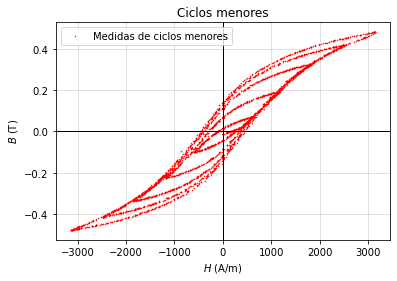
\includegraphics[width=\linewidth]{cincociclos}
	\caption{Ciclos menores del núcleo de hierro}
	\label{fig:cincociclos}
\end{figure}
Se puede observar que las curvas son bastante regulares y mantienene la forma. Esta vez, el núcleo presenta una imanación inicial (aún negativa) bastante menor a la medida anterior. También se puede comprobar que el primer ciclo coincide aproximadamente con el último ciclo de histéresis de los ahora medidos, pues ambos deberían tener la misma amplitud. 
\begin{figure}[ht!]\centering
	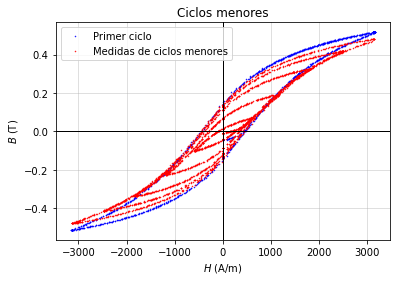
\includegraphics[width=\linewidth]{ciclosciclo}
	\caption{Comparación entre ciclos menores y primer ciclo}
	\label{fig:ciclosciclo}
\end{figure}\\

Como se puede observar en la Figura \ref{fig:ciclosciclo}, los ciclos son muy parecidos. Hay que tener en cuenta las diferencias en las condiciones iniciales de las medidas, así como que las de voltaje suministrado a los circuitos no serán exactamente iguales para ambas medidas, por lo que pueden considerarse resultados satisfactorios. Si ahora se miden los máximos positivos de cada ciclo menor, en este caso a través del Measure, se obtienen una serie de puntos de la curva de conmutación. Estos resultados han sido recogidos en la Tabla \ref{tab:esquizofrenia}.\\

\begin{table}[htb!]
	\centering
	\begin{tabular}{c c c}
		%\hline
		\toprule
		Ciclo & $H$ (A/m)& $B$ (mT) \\
		\midrule[1px]
		1 & 589.372 $\pm$ 0.001  &  70 $\pm$ 1\\
		2 & 1143.161 $\pm$ 0.001  &  195 $\pm$ 1\\
		3 & 1810.826 $\pm$ 0.001  &  327 $\pm$ 1\\
		4 & 2466.542 $\pm$ 0.001  &  414 $\pm$ 1\\
		5 & 3128.891 $\pm$ 0.001 & 481 $\pm$ 1 \\
		\bottomrule
	\end{tabular}
	\caption{Medidas de la curva de conmutación}
	\label{tab:esquizofrenia}
\end{table}

Estos valores pueden representarse junto a la curva de imanación inicial del primer ciclo para facilitar su comparación.

\begin{figure}[ht!]\centering
	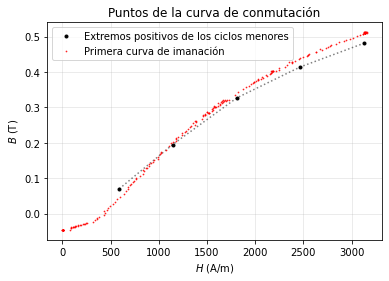
\includegraphics[width=\linewidth]{conmutacion}
	\caption{Curva de conmutación}
	\label{fig:conmutación}
\end{figure}

La Figura \ref{fig:conmutación} muestra que los valores de conmutación empiezan siendo ligeramente superiores a la curva de imanación a campos bajos mientras que a magnitudes de campo externo más elevadas se ven sobrepasados por la misma. Esto, realmente, es un indicador de lo mismo que el solapamiento imperfecto de la Figura \ref{fig:ciclosciclo}. Hay que tener en cuenta que las medidas del primer ciclo así como la de los menores fueron tomadas con una distintas imanación inicial y a amplitudes desiguales, por lo que resulta esperable que no se produzca un solapamiento perfecto de una curva y otra. Sin embargo, es apreciable el hecho de que los máximos de los ciclos menores siguen de cerca la tendencia de la curva de imanación inicial de la medida anterior, por lo que estos resultados pueden considerarse suficientemente satisfactorios. 

\section{Conclusiones}

%------------------------------------------------


%----------------------------------------------------------------------------------------
%	REFERENCE LIST
%----------------------------------------------------------------------------------------

\phantomsection
\bibliographystyle{unsrt}
\bibliography{sample.bib}

%----------------------------------------------------------------------------------------

\end{document}